\section{Theoretical Analysis} \label{section:theo}


\subsection{Node analysis for t$<$0}

\par In this section, a theoretical analysis of the circuit was conducted. The node method was the chosen approach.

The aim of using this method is to determine every node voltage. To do so, the node 4 was considered a reference node. Then, eight independent equations were written in orther to find the remaining unknown node voltage values. Before $t=0s$, v(s) is constant. Therefore, the capacitor behaves like an open-circuit which means Ix=0. The currents in the branches were also computed.


The equations were then put in the form of the matrix shown below. Octave math tools were used to solve the system.



$\begin{bmatrix}
1 & 0 & 0 & 0 & 0 & 0 & 0 & 0\\
-G1 & G1+G2+G3 & -G2 & 0 & -G3 & 0 & 0 & 0\\
0 &-Kb-G2 & G2 & 0 & Kb & 0 & 0 & 0\\
0 & 0 & 0 & 1 & 0 & 0 & 0 & 0\\
0 & -G3 & 0 & -G4 & G3+G4+G5 & -G5 & -G7 & G7\\
0 & Kb & 0 & 0 & -Kb-G5 & G5 & 0 & 0\\
0 & 0 & 0 & -G6 & 0 & 0 & G6+G7 & -G7\\
0 & 0 & 0 & Kd*G6 & -1 & 0 & -Kd*G6 & 1\\
\end{bmatrix}
$$\begin{bmatrix}
V1 \\ V2 \\ V3 \\ V4 \\ V5 \\ V6 \\ V7 \\ V8
\end{bmatrix}$
=
$\begin{bmatrix}
Vs \\ 0 \\ 0 \\ 0 \\ 0 \\ 0 \\ 0 \\ 0
\end{bmatrix}
$

\begin{table}[ht]
  \centering
  \begin{tabular}{|l|r|}
    \hline    
    {\bf Name} & {\bf Value} \\ \hline
    V1 & 5.068716e+00 \\ \hline
V2 & 4.843672e+00 \\ \hline
V3 & 4.369060e+00 \\ \hline
V4 & 0.000000e+00 \\ \hline
V5 & 4.874693e+00 \\ \hline
V6 & 5.579017e+00 \\ \hline
V7 & -1.980764e+00 \\ \hline
V8 & -2.974577e+00 \\ \hline

  \end{tabular}
  \caption{Theoretical nodal voltage results. All variables are expressed in V or A.}
  \label{tab:p2}
\end{table}


\subsection{Calculus of $R_{eq}$}
\label{subsection:2.2}

\par The purpose of this task was to compute the Req (equivalant resistance) of the circuit.

It is known that:
\begin{equation}
R_{eq}=\frac{V_{x}}{I_{x}}
\end{equation}

In order to determine the variable aforementioned, first it was sugested to calculate it seen from the capacitors terminals. Then, using the Thevenin and Norton theorem, we put the independent voltage source to 0V. $V_{x}$ is equivalent to Thevenin's Voltage, and $I_{x}$ to Norton's Current. This is necessary because the depedent voltage short cannot be put equal to 0V(short-circuit) and the independent current source cannot be erased from the circuit.
\par An ilustration of the circuit analysed is showed in figure \ref{sim2draw} 
\begin{figure}[h] \centering
\includegraphics[width=0.65\linewidth]{sim2draw.pdf}
\caption{RC Circuit analysed in section 2.}
\label{sim2draw}
\end{figure}
\par
Then, the values of current of  every branch and the nodal values are obtained using node method. The matrix used in octave is the one that follows.

$\begin{bmatrix}
1 & 0 & 0 & 0 & 0 & 0 & 0 & 0 & 0\\
-G1 & G1+G2+G3 & -G2 & 0 & -G3 & 0 & 0 & 0 & 0\\
0 & -G2-Kb & G2 & 0 & Kb & 0 & 0 & 0 & 0\\
0 & 0 & 0 & 1 & 0 & 0 & 0 & 0 & 0\\
0 & -G1 & 0 & 0 & -G4 & 0 & -G6 & 0 & 0\\
0 & Kb & 0 & 0 & -G5-Kb & G5 & 0 & 0 & 1\\
0 & 0 & 0 & 0 & 0 & 0 & G6+G7& -G7 & 0\\
0 & 0 & 0 & 0 & 0 & 1 & 0 & -1 & 0\\
0 & 0 & 0 & KdG6 & -1 & 0 & -Kd*G6 & 1 & 0
\end{bmatrix}$
$\begin{bmatrix}
V1 \\ V2 \\ V3 \\ V4 \\ V5 \\ V6 \\ V7 \\ V8 \\ I_{x}
\end{bmatrix}$
= 
$\begin{bmatrix}
0 \\ 0 \\ 0 \\ 0 \\ 0 \\ 0 \\ 0 \\ V_{x} \\ 0
\end{bmatrix}$

\par Theoretically speaking, once the voltage source is equal to 0V, $V_{4}$ and  $V_{1}$ are also to be 0. 

\begin{table}[]
  \centering
  \begin{tabular}{|l|r|}
    \hline    
    {\bf Name} & {\bf Value} \\ \hline
    V1 & 0.000000e+00 \\ \hline
V2 & 0.000000e+00 \\ \hline
V3 & 9.496396e-16 \\ \hline
V4 & 0.000000e+00 \\ \hline
V5 & 5.935248e-17 \\ \hline
V6 & 8.553593e+00 \\ \hline
V7 & -2.967624e-17 \\ \hline
V8 & 0.000000e+00 \\ \hline
Ix & -2.745419e-03 \\ \hline
Req & 3.115588e+03 \\ \hline
tau & 3.244185e-03 \\ \hline

  \end{tabular}
  \caption{Theoretical nodal voltage results. All variables are expressed in Volt, Ampere or Ohm.}
  \label{tab:p2}
\end{table}


\clearpage

\subsection{Node analysis for t $\ge$ 0 (Natural solution)}


It was proposed to study and determine the natural response of the circuit over time, in node 6. The natural response is what the circuit does including the initial conditions (initial voltage of the capacitor) but with the imput supressed. 

In order to calculate the natural solution, we have to eliminate the voltage source, which means vs(t)=0V. Hence, we have an equivalent cicuit described by a voltage source and the capacitor. The current flowing through the capacitor is in fact consumed by it. Therefore, the voltage V8=0V and the amplitude $Vx=V6-V8=V6$.The natural solution will have the format $V{6n}(t)=A*e^{(-t/tau)}$ with $tau=Req*C$ and $A=V6$ obtained in \ref{subsection:2.2}. As expected, the result is a negative exponencial graph, shown bellow.

\begin{figure}[ht] \centering
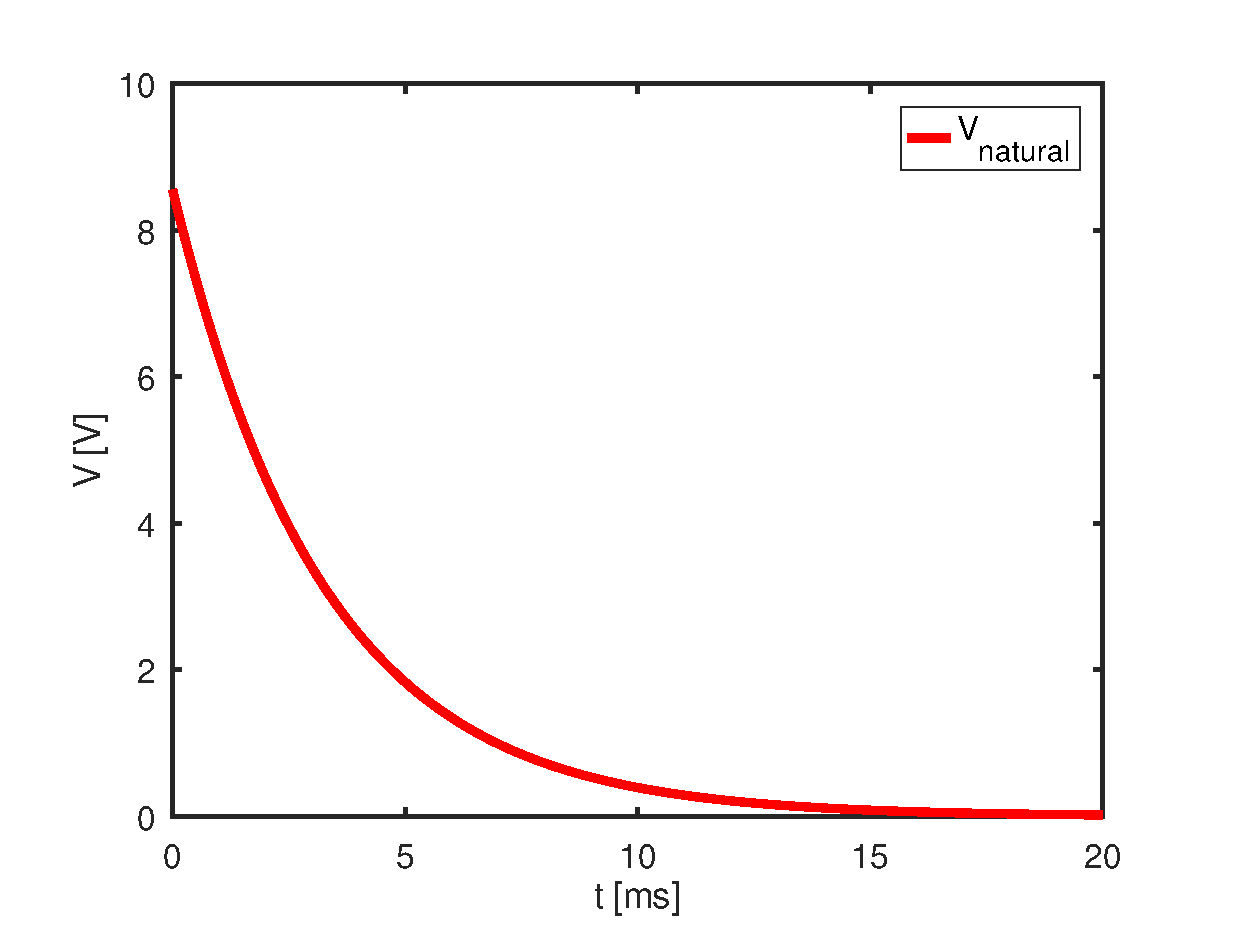
\includegraphics[width=0.5\linewidth]{natural.eps}
\caption{Circuit analysed.}
\label{fig:sim3}
\end{figure}



\subsection{Node analysis for t $\ge$ 0 (Forced solution)}

The forced response of a circuit is calculated with the sources turned on, but with the initial conditions (internal stored energy) set to zero.What is forced response? The forced response is where the output (the voltage on the capacitor) is going to end up in the long run after all stored energy eventually dissipates. The forced response does this by ignoring the presence of energy storage elements (in this case, it ignores the capacitor and its initial voltage). However, the forced response can't tell us what happens at t=0, or during the transition to the final state, because it ignores the stored energy. 
\par Like so, a phasor was used, with $V_{s}=1$. The capacitor was replaced by its impiedence $Z$. Then, the nodal method was run again, with this new variable.
\begin{equation}
w=2*pi*f
\end{equation} 

\begin{equation}
Zc=1/(j*w*C);
\end{equation} 

\par The matrix used was the following:

$\begin{bmatrix}
1 & 0 & 0 & -1 & 0 & 0 & 0 & 0 \\
-G1 & G1+G2+G3 & -G2 & 0 & -G3 & 0 & 0 & 0 \\
0 & -G2-Kb & G2 & 0 & Kb & 0 & 0 & 0 \\
0 & 0 & 0 & 1 & 0 & 0 & 0 & 0 \\
0 & G3 & 0 & G4 &-G3-G5-G4 & G5+1/Zc & G7 & -G7-1/Z_{c}\\
0 & Kb & 0 & 0 & -G5-Kb & G5+1/Z_{c} & 0 & -1/Z_{c} \\
0 & 0 & 0 & 0 & 0 & 0 & G6+G7& -G7 \\
0 & 0 & 0 & KdG6 & -1 & 0 & -Kd*G6 & 1
\end{bmatrix}$
$\begin{bmatrix}
V1 \\ V2 \\ V3 \\ V4 \\ V5 \\ V6 \\ V7 \\ V8
\end{bmatrix}$
= 
$\begin{bmatrix}
1 \\ 0 \\ 0 \\ 0 \\ 0 \\ 0 \\ 0 \\ 0 \\ 
\end{bmatrix}$
\par Then, the complex amplitudes with the knowlegde that the amplitude of the forced response is the absolute value of the complex $V_{6}$, and the phase is the argument, the forced solution is then given by:

\begin{equation}
V6_f=A*sin(w*t+Ph)
\end{equation} 

\par The tables below present the values that allows us to compute the comlex amplitude of every node voltage. In fact, it is obtained by the following expression: 

\begin{equation}
V_{complex}(i)=V_i exp(-j*phase(i))
\end{equation} 


\begin{table}[ht]

  \centering
  \begin{tabular}{|l|r|}
    \hline    
    {\bf Name} & {\bf Value [V]} \\ \hline
    V1 & 1.000000e+00 \\ \hline
V2 & 9.556014e-01 \\ \hline
V3 & 8.619659e-01 \\ \hline
V4 & 2.801649e-17 \\ \hline
V5 & 9.617215e-01 \\ \hline
V6 & 5.886212e-01 \\ \hline
V7 & 3.907822e-01 \\ \hline
V8 & 5.868501e-01 \\ \hline

  \end{tabular}
  \caption{Amplitudes of Nodal Voltages} 
\end{table}


\begin{table}[ht]

  \centering
  \begin{tabular}{|l|r|}
    \hline    
    {\bf Name} & {\bf Value [Rad]} \\ \hline
    Phase1 & 0.000000e+00 \\ \hline
Phase2 & -5.722643e-16 \\ \hline
Phase3 & -1.142921e-15 \\ \hline
Phase4 & 3.141593e+00 \\ \hline
Phase5 & -5.388346e-16 \\ \hline
Phase6 & -3.000819e+00 \\ \hline
Phase7 & 3.141593e+00 \\ \hline
Phase8 & 3.141593e+00 \\ \hline

  \end{tabular}
  \caption{Phase of Nodal Voltages} 
\end{table}




\newpage



\subsection{Natural and Forced Superimposed}


The total response of a circuit can be teased apart into a forced response plus a natural response. These responses can be combined using the principle of superposition. This principle pressupose the addition of the natural response and the forced response, both calculated in question 3 and 4.

The final solution for $V(6)_{final}$  is then given by:


\begin{equation}
V6_{final}
\begin{cases}
V_{6}-V_{8} & $t$ < $0$ \\
V(6)_{n} + A*sin(w*t+Ph) & $t $\geq$ 0$
\end{cases}
\label {eq:n2}
\end{equation}



The final solution for $V(S)_{final}$  is then given by:

\begin{equation}
VS_{final}
\begin{cases}
Vs & $t$ < $0$ \\
e.^(-j*(w*t_pos-pi/2))& $t $\geq$ 0$
\end{cases}
\label {eq:n2}
\end{equation}


\begin{figure}[h] \centering
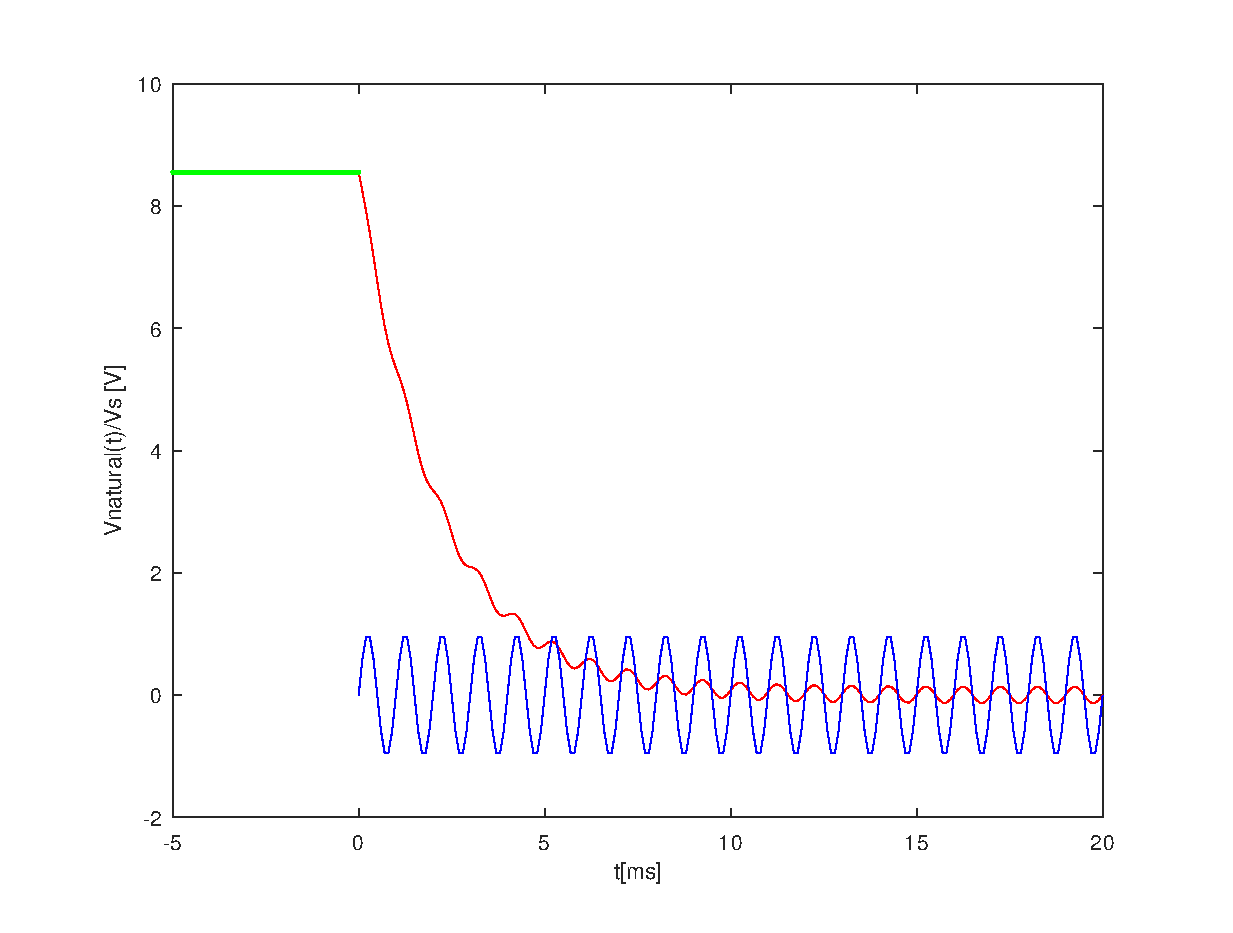
\includegraphics[width=0.6\linewidth]{part4.eps}
\caption{Final response.}
\label{fig:part4}
\end{figure}

\par It is observed in \ref{fig:part4} that $V(6)_{final}$ tends to diminuish  until 20ms, the end of the period. By this time, the phase $V(6)_{final}$ and the phase of  $VS_{final}$ differ $\pi$ or 180 degrees.




\subsection{Frequency Responses}

In this section, both octave and ngspice were used in order to obtain plots of the phase response and of the magnitude response, using logscale. This approach is very useful hence it provides a much better plot fit and, therefore it provides great visualization for users. The magnitude in debicels is of interest for analysis of sound waves, and the analysis of the phase or angle delay is a very interesting way of study another parameter to compare signal. Frequency range in both analysis was from 0.1 Hz to 1MHz. The plots made were v6(f), vs(f) and vc=(v6(f)-v8(f)).



To examine the frequency responses, the system of equations in Section 4 is solved in a loop cycle, what allows us to calculate the $V_6$, $V_c$ and $V_s$ for each frequence. For each result of these complex vectors, the values were saved.

\subsubsection{Frequency Response- Magnitude}

To represent the magnitude in dB, the absolute values were converted ($X_{dB}$=20$log_{10}$(X)). The frequencies were put in a logarithmic scale.

The magnitude of $V_s$ does not suffer any alteration with the variation of the frequency of the signal. Since its amplitude is 1, as one can observe in the graphics shown at the end of the section, the plot shows a constant horizontal line, with the value zero (0=$log_{10}$(1)).

On the contrary, as the frequency is increasing, the magnitudes of $V_6$ and $V_c$ decrease. The value of $V_c$ changes as it is expected in a RC circuit. This is due to the impedance of the capacitor (Z=-j/wC).

\begin{figure}[h] \centering
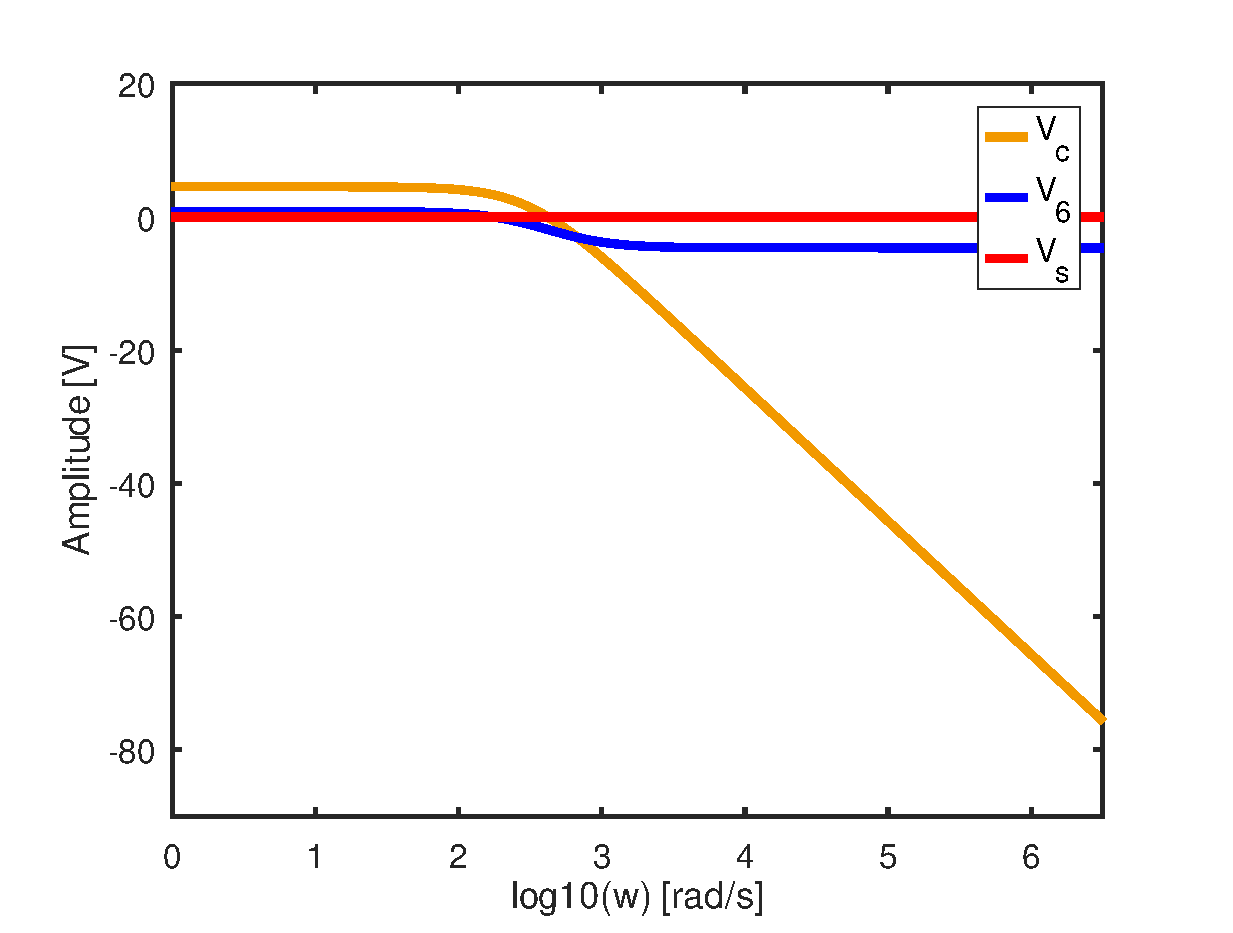
\includegraphics[width=0.5\linewidth]{part6_amp.eps}
\caption{Circuit analysed.}
\label{Magnitude response.}
\end{figure}

\subsubsection{Frequency Response- Phase}


The angles of the values saved were transformed from radians to degrees. The phase in $V_s$ is 0, therefore we do not have to do any further calculations. The phase of each voltage corresponds to the exact angles. In the plot shown below, the frequencies were also  put in the logarithmic scale. As the frequency increases the phase tend to negative values, which varies as it is expected.

\begin{figure}[ht] \centering
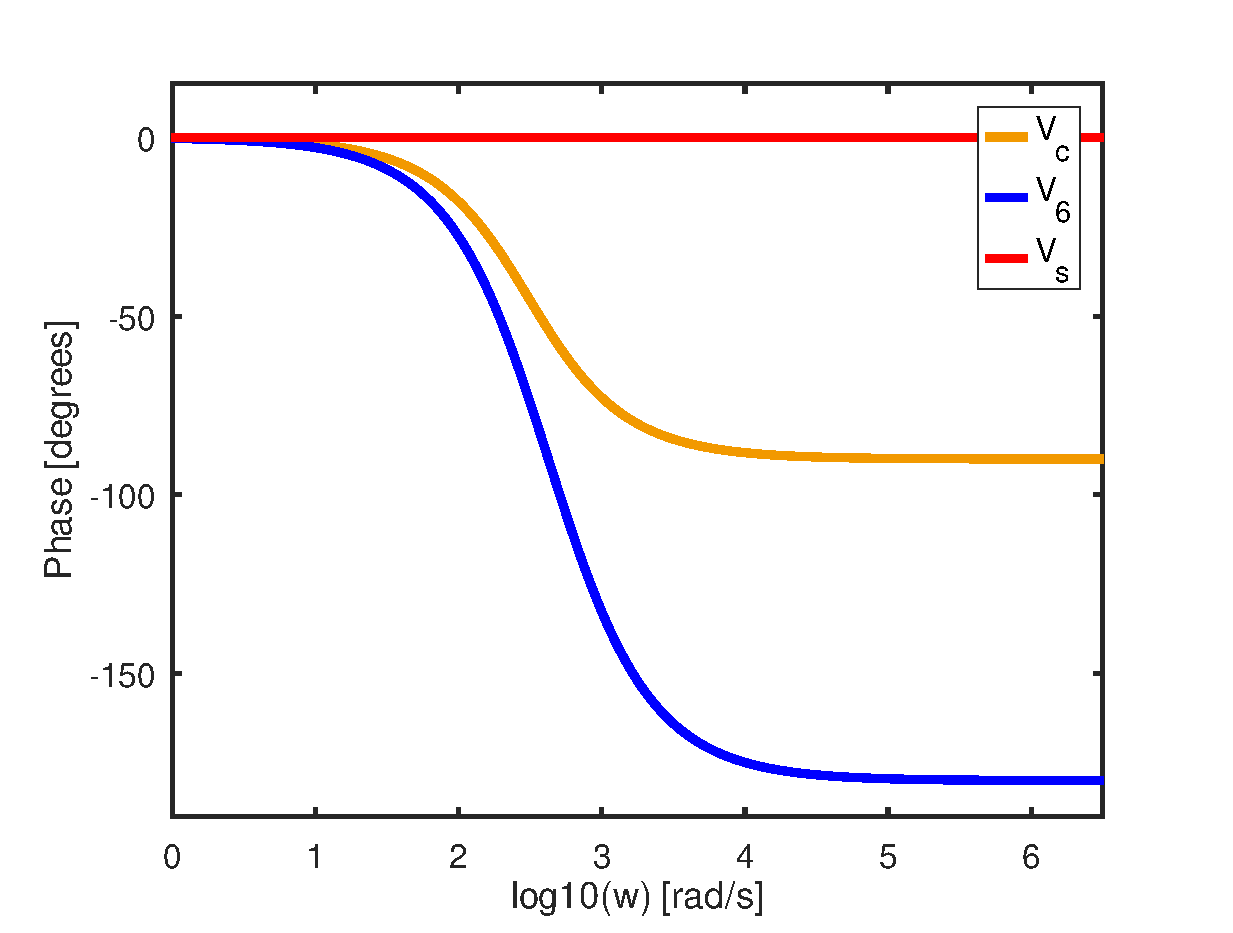
\includegraphics[width=0.5\linewidth]{part6_ang.eps}
\caption{Phase response.}
\label{RC Circuit.}
\end{figure}













